\documentclass{ctexart}
\usepackage[left=1.5cm,right=1.5cm,top=1.5cm,bottom=1.5cm]{geometry}
\usepackage{listings}
\usepackage[dvipsnames]{xcolor}
\usepackage{cite}
\usepackage{diagbox}
\usepackage{fancyhdr} % 加载fancyhdr宏包,用于设置页眉和页脚
\pagestyle{fancy} % 设置页面样式
\fancyhf{} % 清除默认的页眉和页脚的内容
\fancyfoot[C]{\thepage} 
\renewcommand{\headrulewidth}{0pt} % 将页眉的横线宽度设置为0pt

\usepackage{graphicx}
\usepackage{longtable}
\usepackage{tabularx}
\usepackage{float}
\usepackage{amsmath}%引用宏包要放在documentclass后面,否则报错
\usepackage{hyperref}
\usepackage{bm}
\usepackage{amssymb}
\usepackage{esint}
\usepackage{booktabs}
%\usepackage{subfiles}%用于分章节管理引用,使各章节引用来源于各自的文件,编号相互独立
\usepackage{amsthm}
\title{数字电路实验\quad 实验报告7}
\author{Leo}
\date{\today}

\begin{document}
\maketitle
\section{实验内容}
使用74194构成不少于3位的自启动环形计数器和扭环计数器:

1.熟悉74194芯片

2.列出状态转移真值表和转换图 

3.给出电路实现方案

4.调试电路,实现环形计数器和扭环计数器

5.检查自启动

\section{实验器材}
Pocketlab、电脑、导线若干、镊子、限流电阻2个、红色LED灯2个、7400*2、7404*1、74194*2。部分芯片的引脚图如下所示
\begin{figure}[H]
    \centering
    \begin{minipage}{0.5\textwidth}
    \centering
           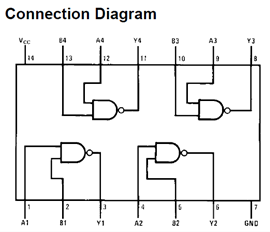
\includegraphics[width=0.6\textwidth]{7400.png}
           \caption{7400}
    \label{}
    \end{minipage}
    \hspace{0.05\textwidth}
    \begin{minipage}{0.3\textwidth}
    \centering
           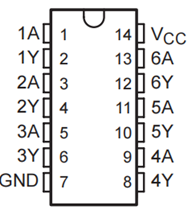
\includegraphics[width=0.6\textwidth]{7404.png}
           \caption{7404}
    \label{7474}
    \end{minipage}
\end{figure}

\begin{figure}[H]
    \centering
    \begin{minipage}{0.5\textwidth}
    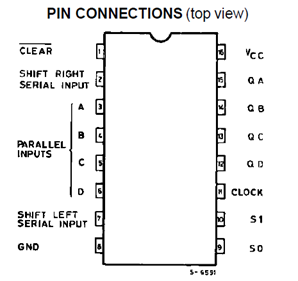
\includegraphics[width=0.4\textwidth]{74194.png}
           \caption{74194}
    \label{}
    \end{minipage}
    \hspace{0.05\textwidth}
    \begin{minipage}{0.3\textwidth}
    
    \end{minipage}
\end{figure}
\section{实验原理}
为了设计三位环形计数器和三位扭环计数器,首先应该确定主循环的状态。列出下表所示的状态转移真值表
\begin{table}[H]
    \centering
    \caption{三位环形计数器的状态转移真值表}
    \begin{tabular}{ccccccc}
    \hline 
        $Q_0^n$ & $Q_1^n$ & $Q_2^n$ & $Q_0^{n+1}$ & $Q_1^{n+1}$ & $Q_2^{n+1}$ & $Z$\\ \hline 
        0 & 0 & 1 & 1 & 0 & 0 & 1\\
        1 & 0 & 0 & 0 & 1 & 0 & 0\\ \hline
        0 & 1 & 0 & 0 & 0 & 1 & 0\\
    \end{tabular}
    \label{状态转移真值表}
\end{table}
规定了当$Q_0Q_1Q_2=001$时输出高电平。
可以写出对应的状态转移方程
\begin{equation}\label{1}
    D_{SR}=Q_2^{n}
\end{equation}
检查电路是否能自启动。按照式\ref{1}可以得到偏离状态的转移次态。以此做出所有状态的转换图
\begin{figure}[H]
    \centering
    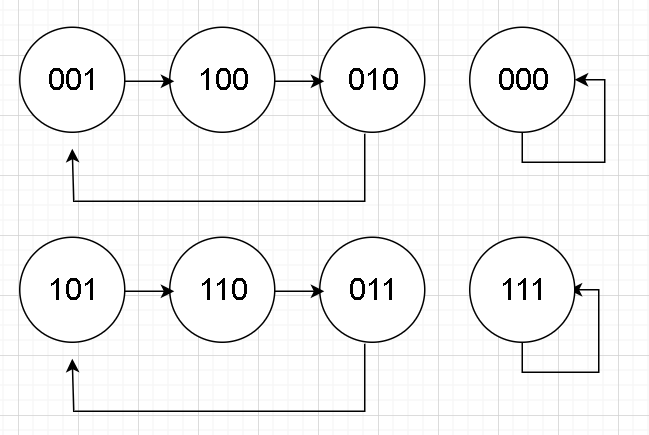
\includegraphics[width=0.4\textwidth]{环形不能自启动.png}
\end{figure}
为了将偏离状态改正到主循环且不改变原有的状态,可以做如下修正
\begin{enumerate}
    \item 011变为001
    \item 000变为100
    \item 111变为011
\end{enumerate}
状态转移方程随之改为
\begin{align}
    D_{SR}&=Q_2\cdot (Q_0'Q_1Q_2)'\cdot (Q_0Q_1Q_2)'+Q_0'Q_1'Q_2'\\
          &=Q_2(Q_0+Q_1'+Q_2')(Q_0'+Q_1'+Q_2')+Q_0'Q_1'Q_2'\\
          &=Q_1'(Q_2+Q_0')\\
          &=((Q_2Q_1')'\cdot (Q_0'Q_1')')
\end{align}
修正后的状态转换图为
\begin{figure}[H]
    \centering
    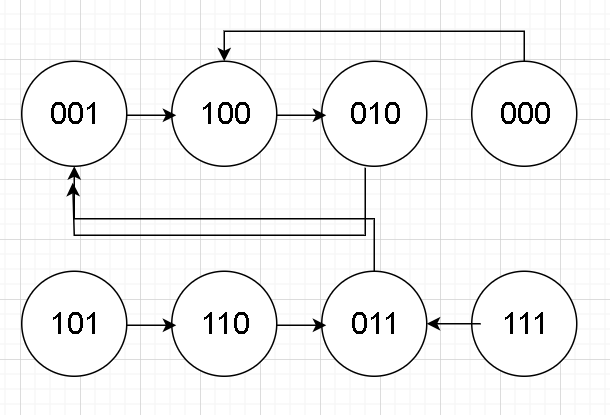
\includegraphics[width=0.4\textwidth]{环形能自启动.png}
\end{figure}
因为一个周期内只有一个1出现,所以可以将$D_{SR}$直接作为输出,满足要求。

下面考察扭环计数器。列出下表所示的状态转移真值表
\begin{table}[H]
    \centering
    \caption{三位扭环计数器的状态转移真值表}
    \begin{tabular}{ccccccc}
    \hline 
        $Q_0^n$ & $Q_1^n$ & $Q_2^n$ & $Q_0^{n+1}$ & $Q_1^{n+1}$ & $Q_2^{n+1}$ & $Z$\\ \hline 
        0 & 0 & 0 & 1 & 0 & 0 & 0\\
        1 & 0 & 0 & 1 & 1 & 0 & 0\\
        1 & 1 & 0 & 1 & 1 & 1 & 1\\
        1 & 1 & 1 & 0 & 1 & 1 & 0\\ 
        0 & 1 & 1 & 0 & 0 & 1 & 0\\ 
        0 & 0 & 1 & 0 & 0 & 0 & 0\\ \hline
    \end{tabular}
    \label{状态转移真值表}
\end{table}
规定了当$Q_0Q_1Q_2=111$时输出高电平。
可以写出对应的状态转移方程
\begin{equation}\label{1}
    D_{SR}=Q_2'^{n}
\end{equation}
依照上式可以得到所有状态的转换图
\begin{figure}[H]
    \centering
    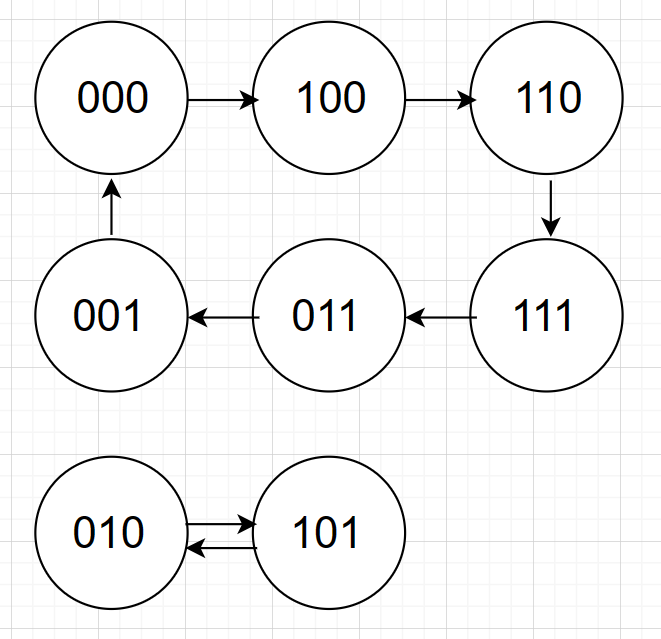
\includegraphics[width=0.3\textwidth]{不能自启动.png}
\end{figure}
发现电路不能自启动,同样需要修正。考虑将101的次态变为110,则状态转移方程修改为
\begin{align}
    D_{SR}&=Q_2'+Q_0Q_1'Q_2\\
    &=Q_2'+Q_0Q_1'\\
    &=(Q_2\cdot (Q_0Q_1')')'
\end{align}
修改后的状态转换图为
\begin{figure}[H]
    \centering
    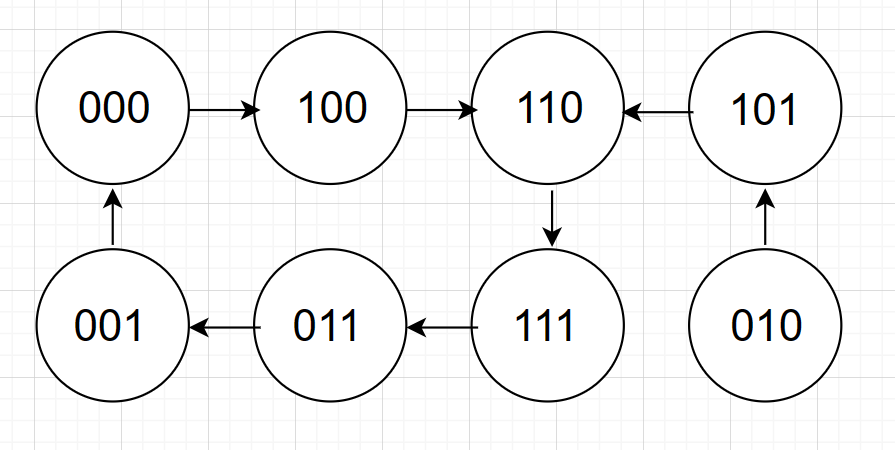
\includegraphics[width=0.4\textwidth]{自启动.png}
\end{figure}
因为扭环计数器一个周期内出现多个1和多个0,所以不能像环形计数器一样直接将$D_{SR}$接到输出,需要专门构造输出函数。为了将$Q_0Q_1Q_2=111$输出为1,并只用与非门和非门,现做如下变形
\begin{align}
    Q_0Q_1Q_2&=((Q_0Q_1)'+Q_3')\\
    &=((Q_0Q_1)''\cdot Q_2)''
\end{align}
\section{电路实现与调试}
在Multisim中搭建上文所述的电路
\begin{figure}[H]
    \centering
    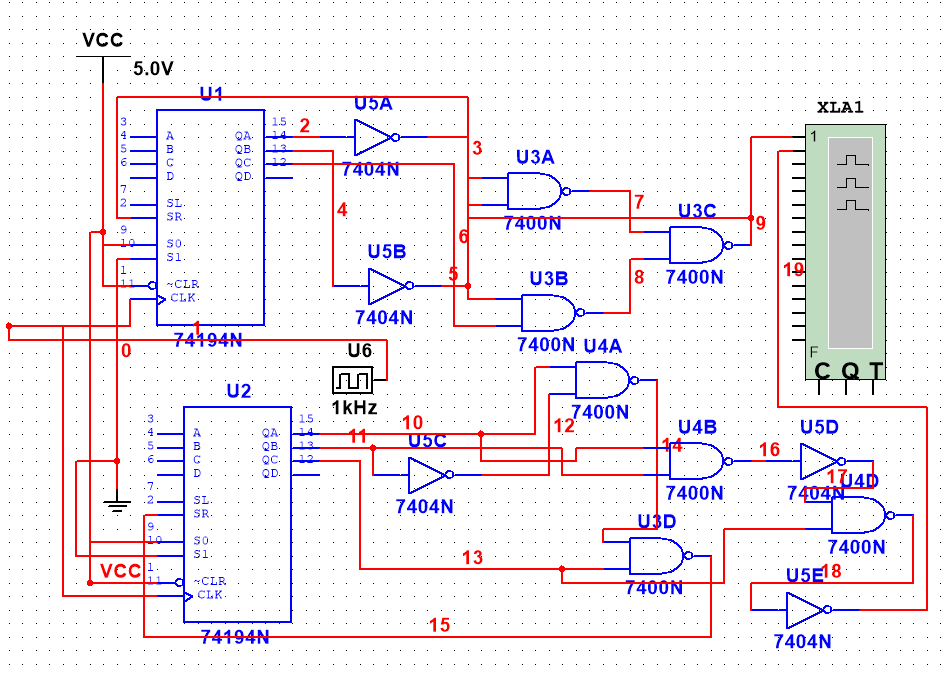
\includegraphics[width=0.6\textwidth]{multisim.png}
\end{figure}
同时对两个计数器进行测试,得到的逻辑分析仪结果如下图所示
\begin{figure}[H]
    \centering
    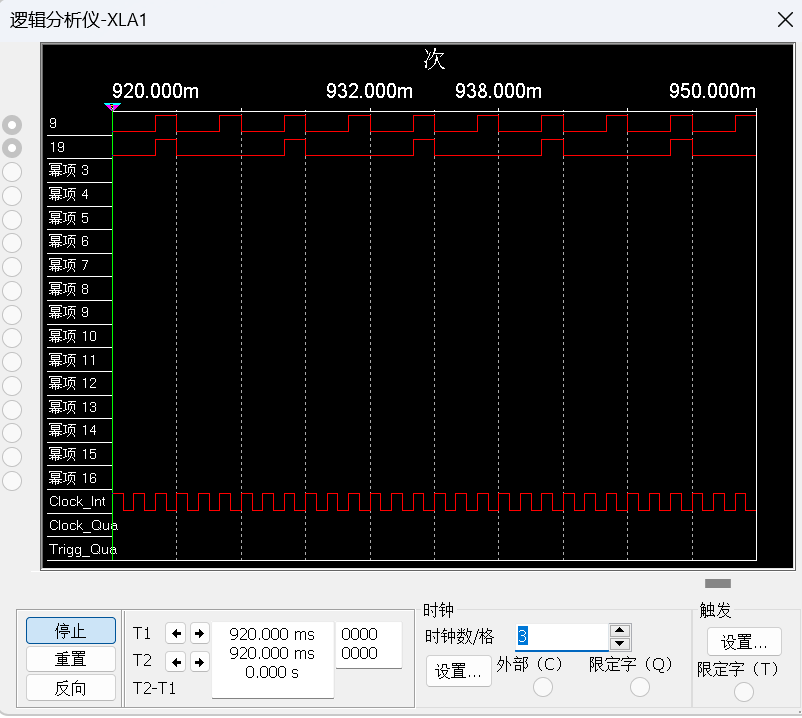
\includegraphics[width=0.5\textwidth]{逻辑分析仪.png}
\end{figure}
可以看到,环形计数器每3个时钟输出一个高电平,扭环计数器每6个时钟输出一个高电平,符合要求。下面搭建实物电路
\begin{figure}[H]
    \centering
    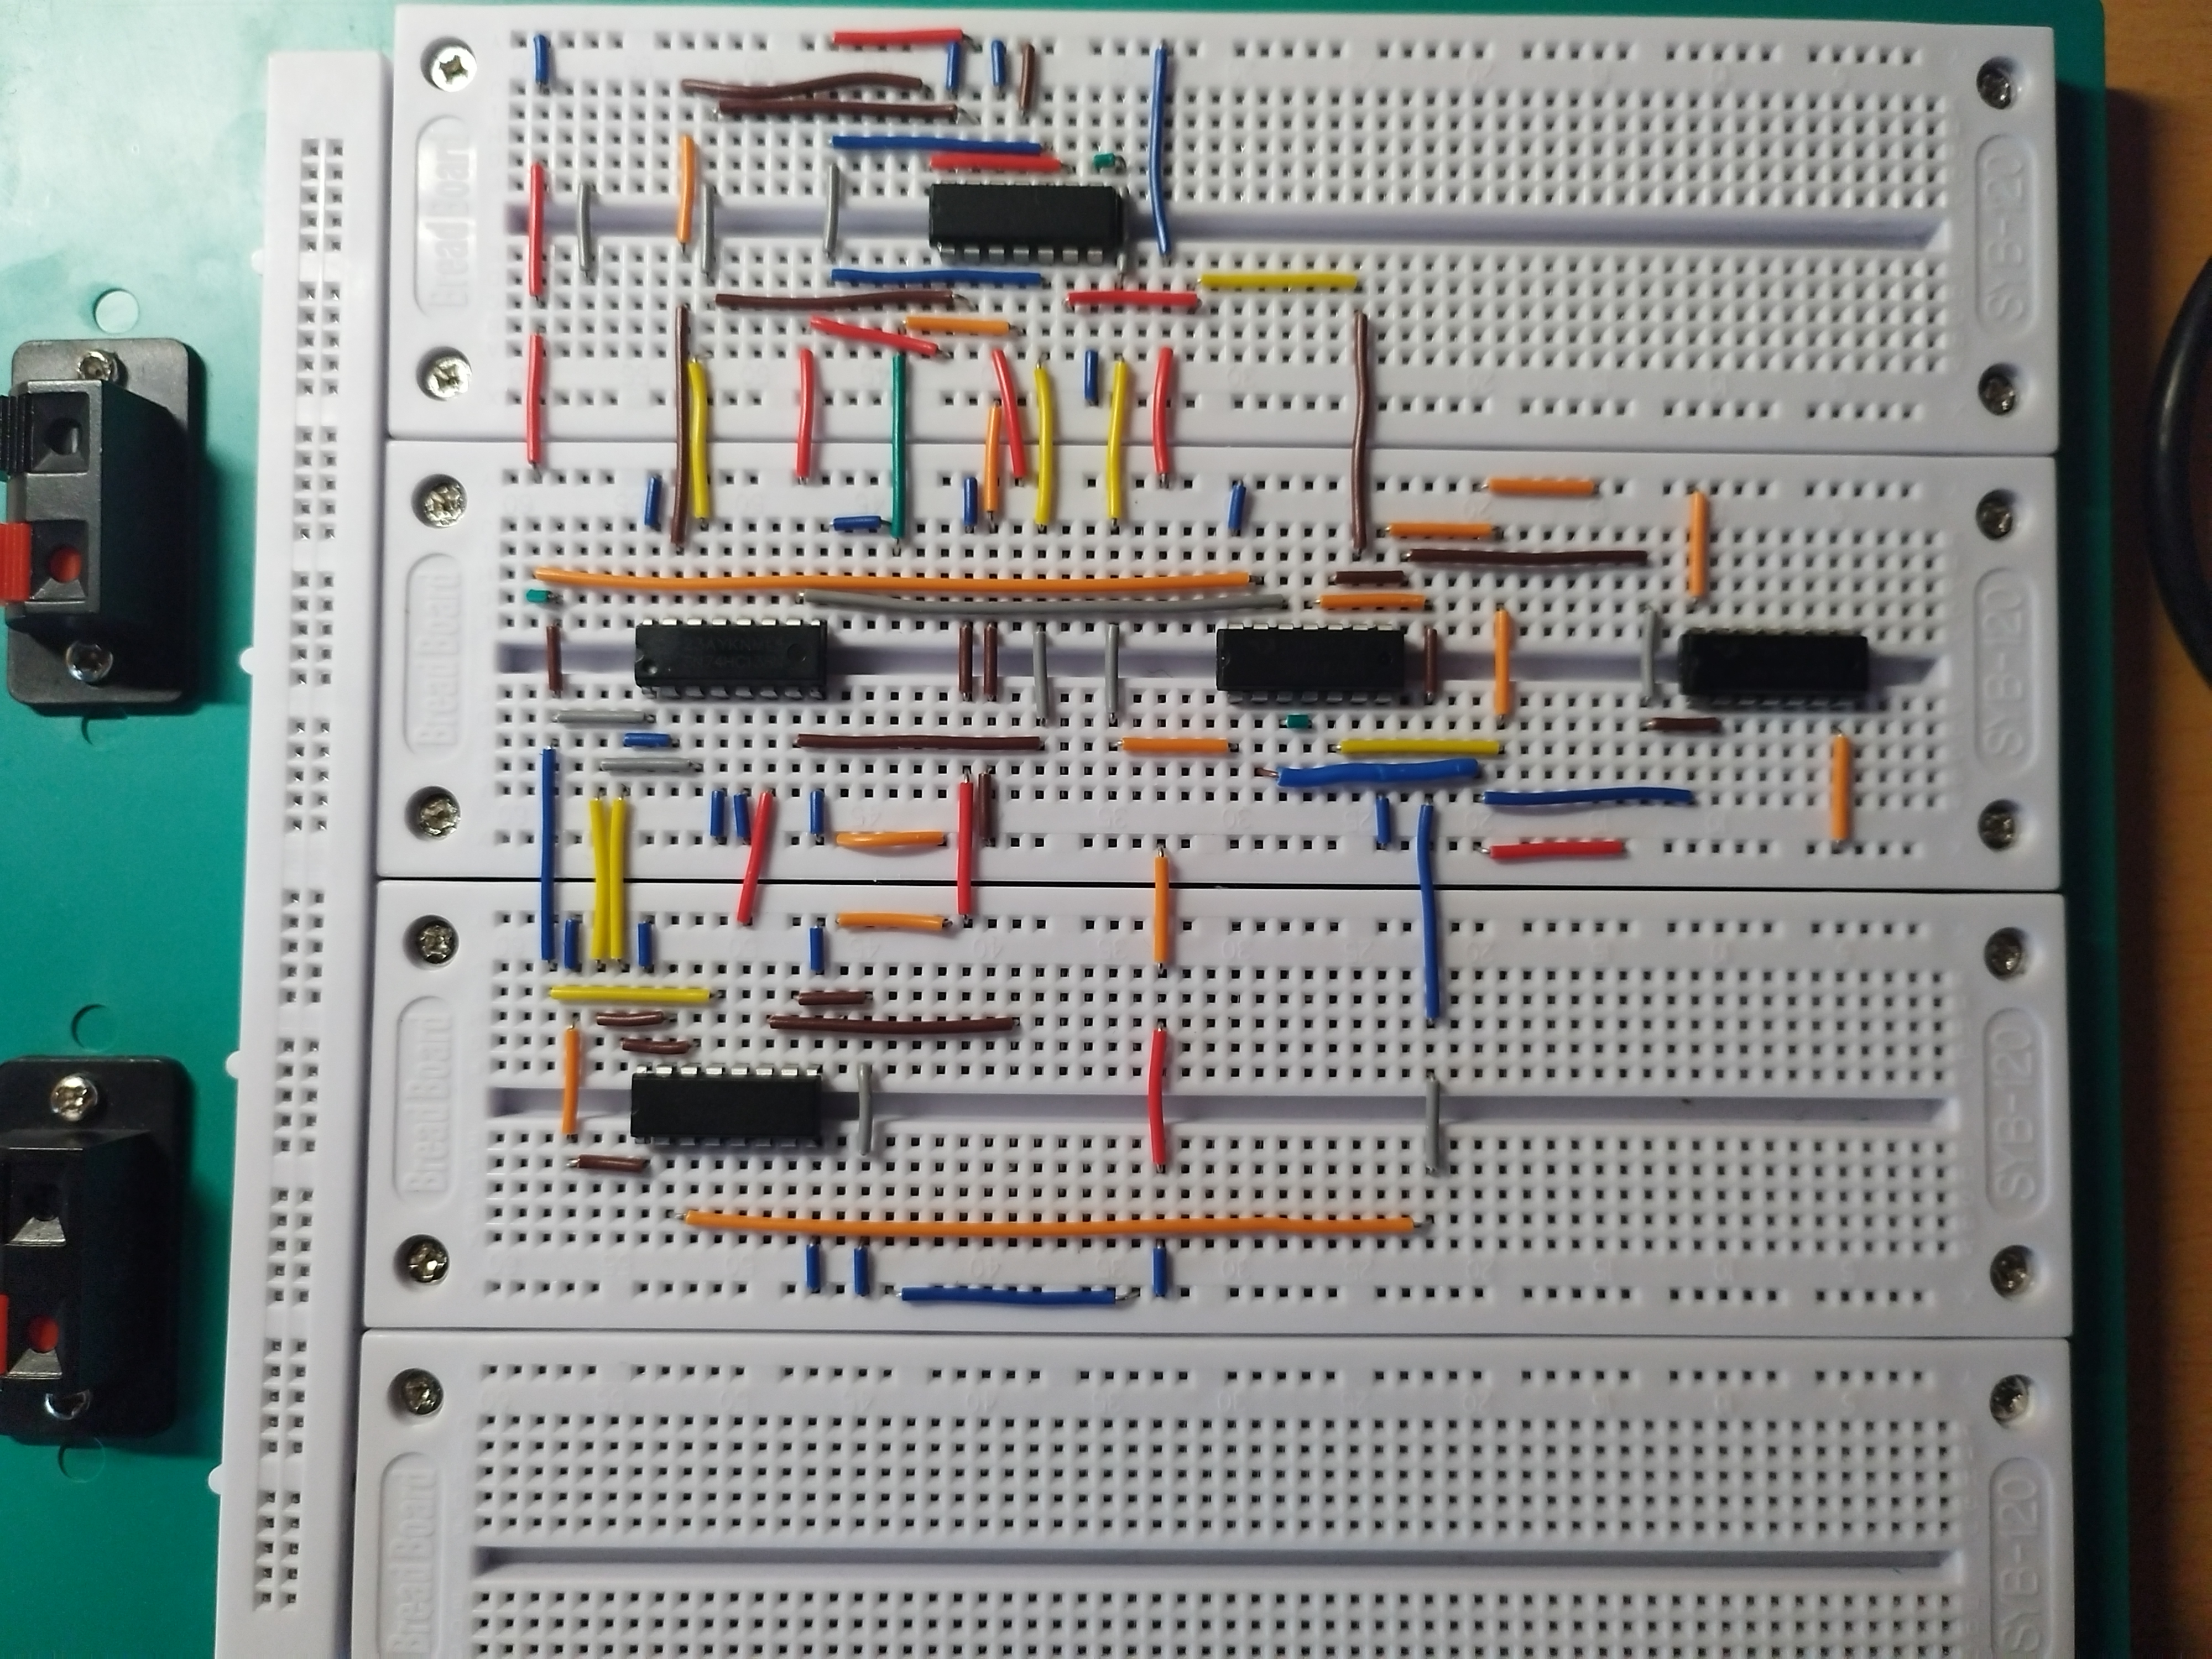
\includegraphics[width=0.5\textwidth]{实物图.jpg}
\end{figure}
上电测试,使用pocketlab逻辑分析仪,可以看到环形计数器每三个时钟出现一个高电平,扭环计数器每六个时钟出现一个高电平
\begin{figure}[H]
    \centering
    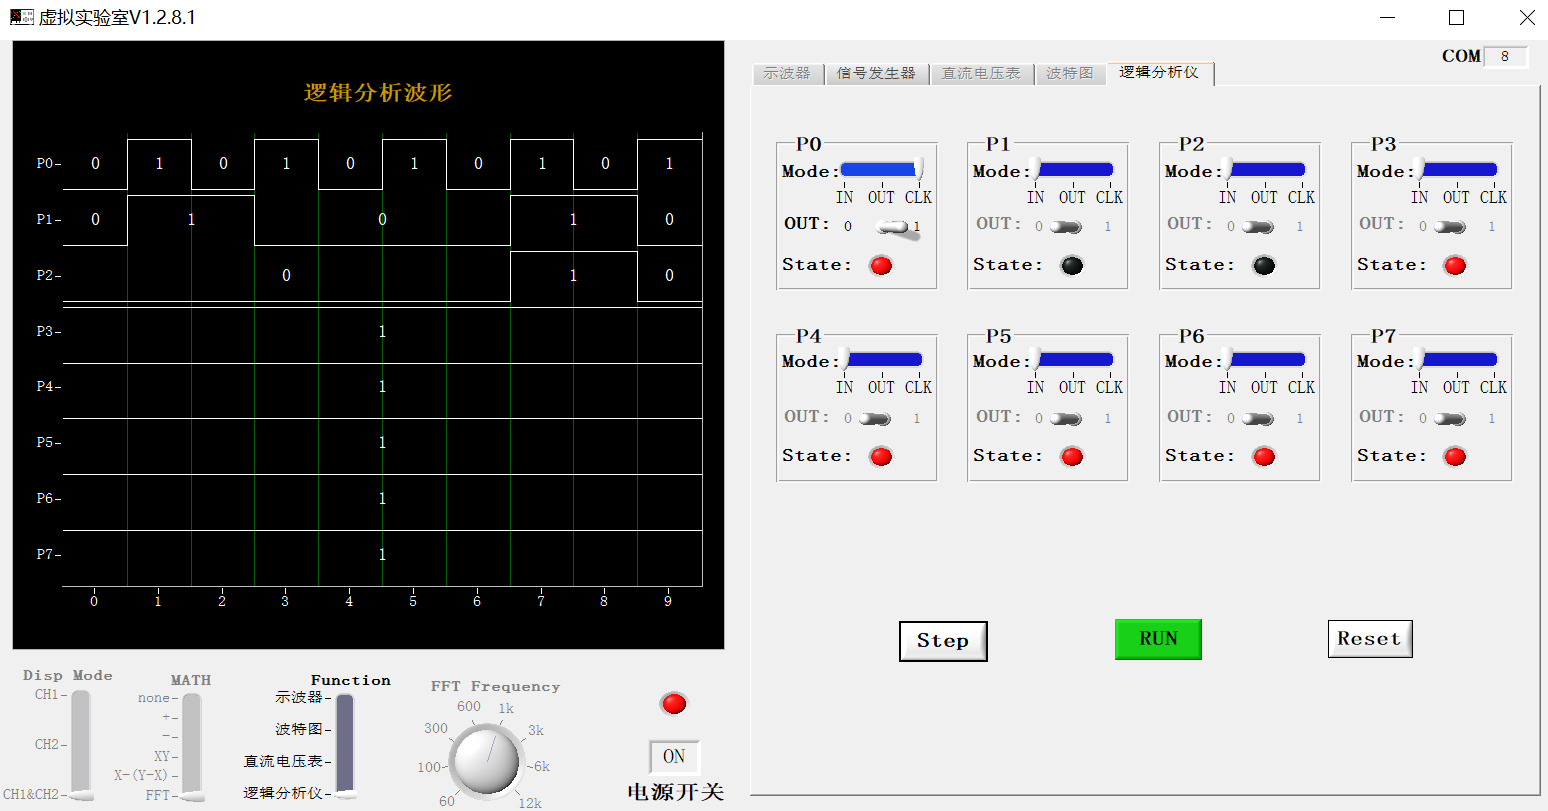
\includegraphics[width=0.5\textwidth]{pocketlab.png}
\end{figure}
下面两图是用LED灯指示计数的实物图
\begin{figure}[H]
    \centering
    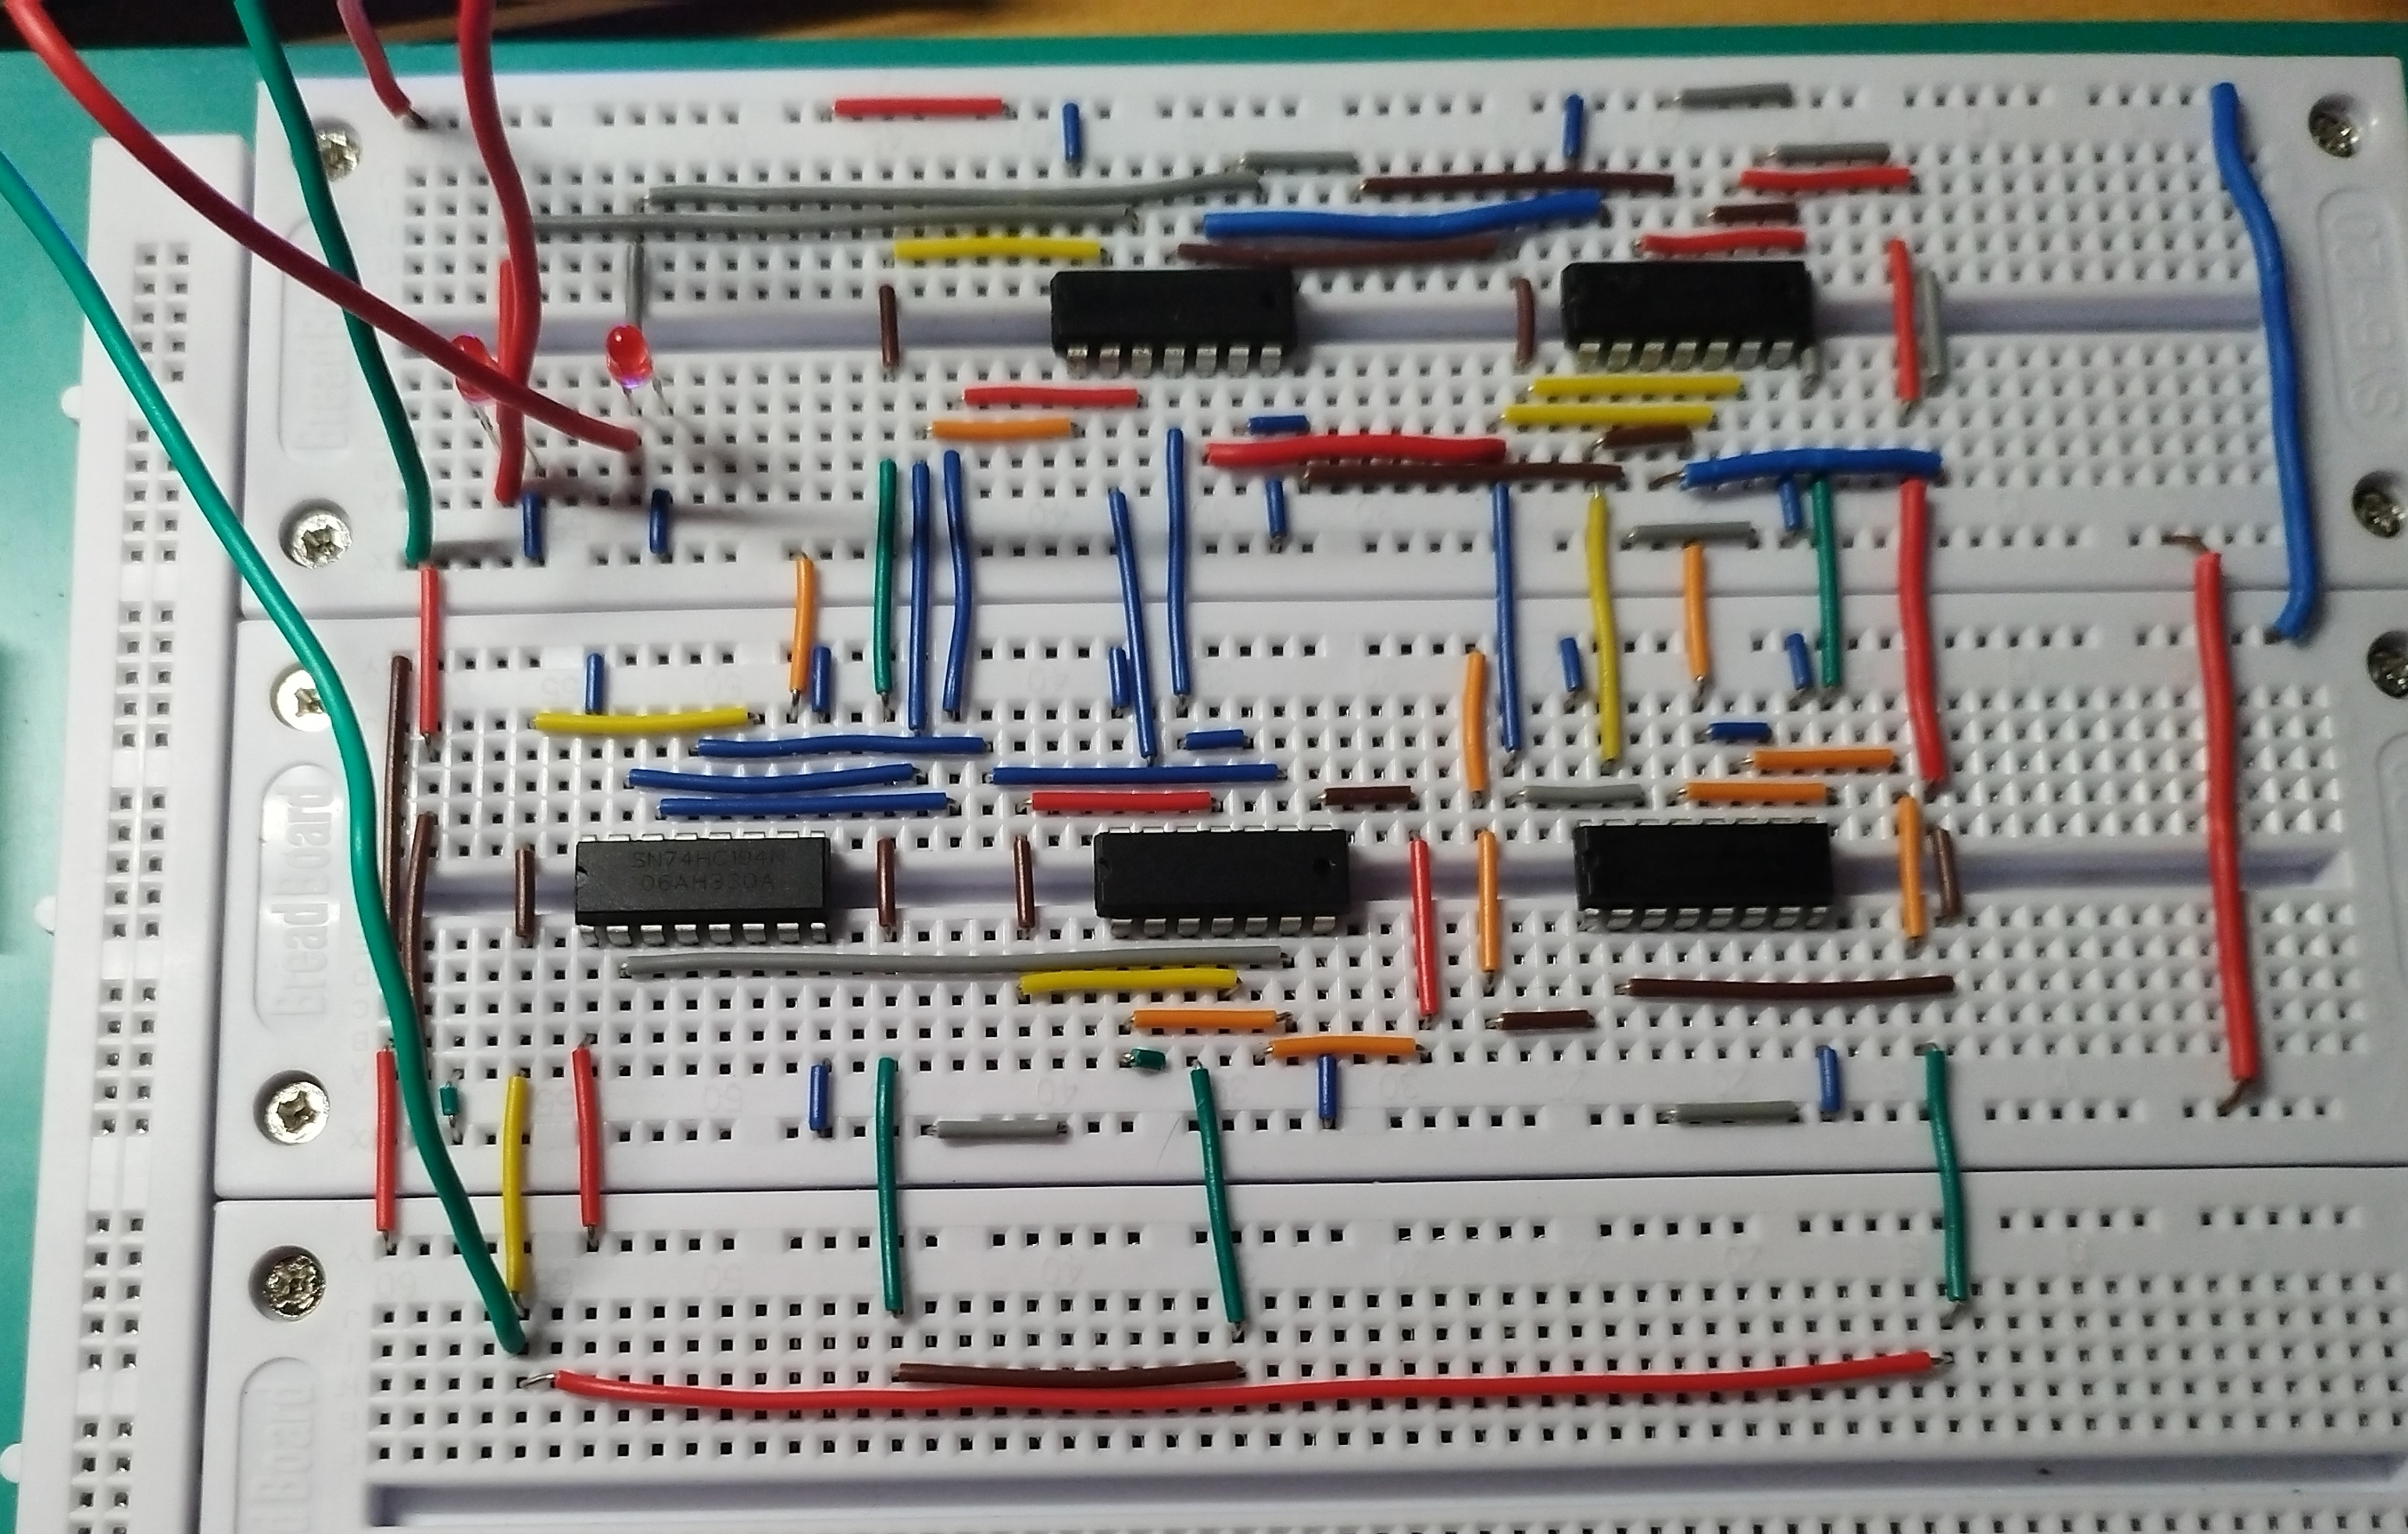
\includegraphics[width=0.5\textwidth]{不亮.jpg}
\end{figure}
\begin{figure}[H]
    \centering
    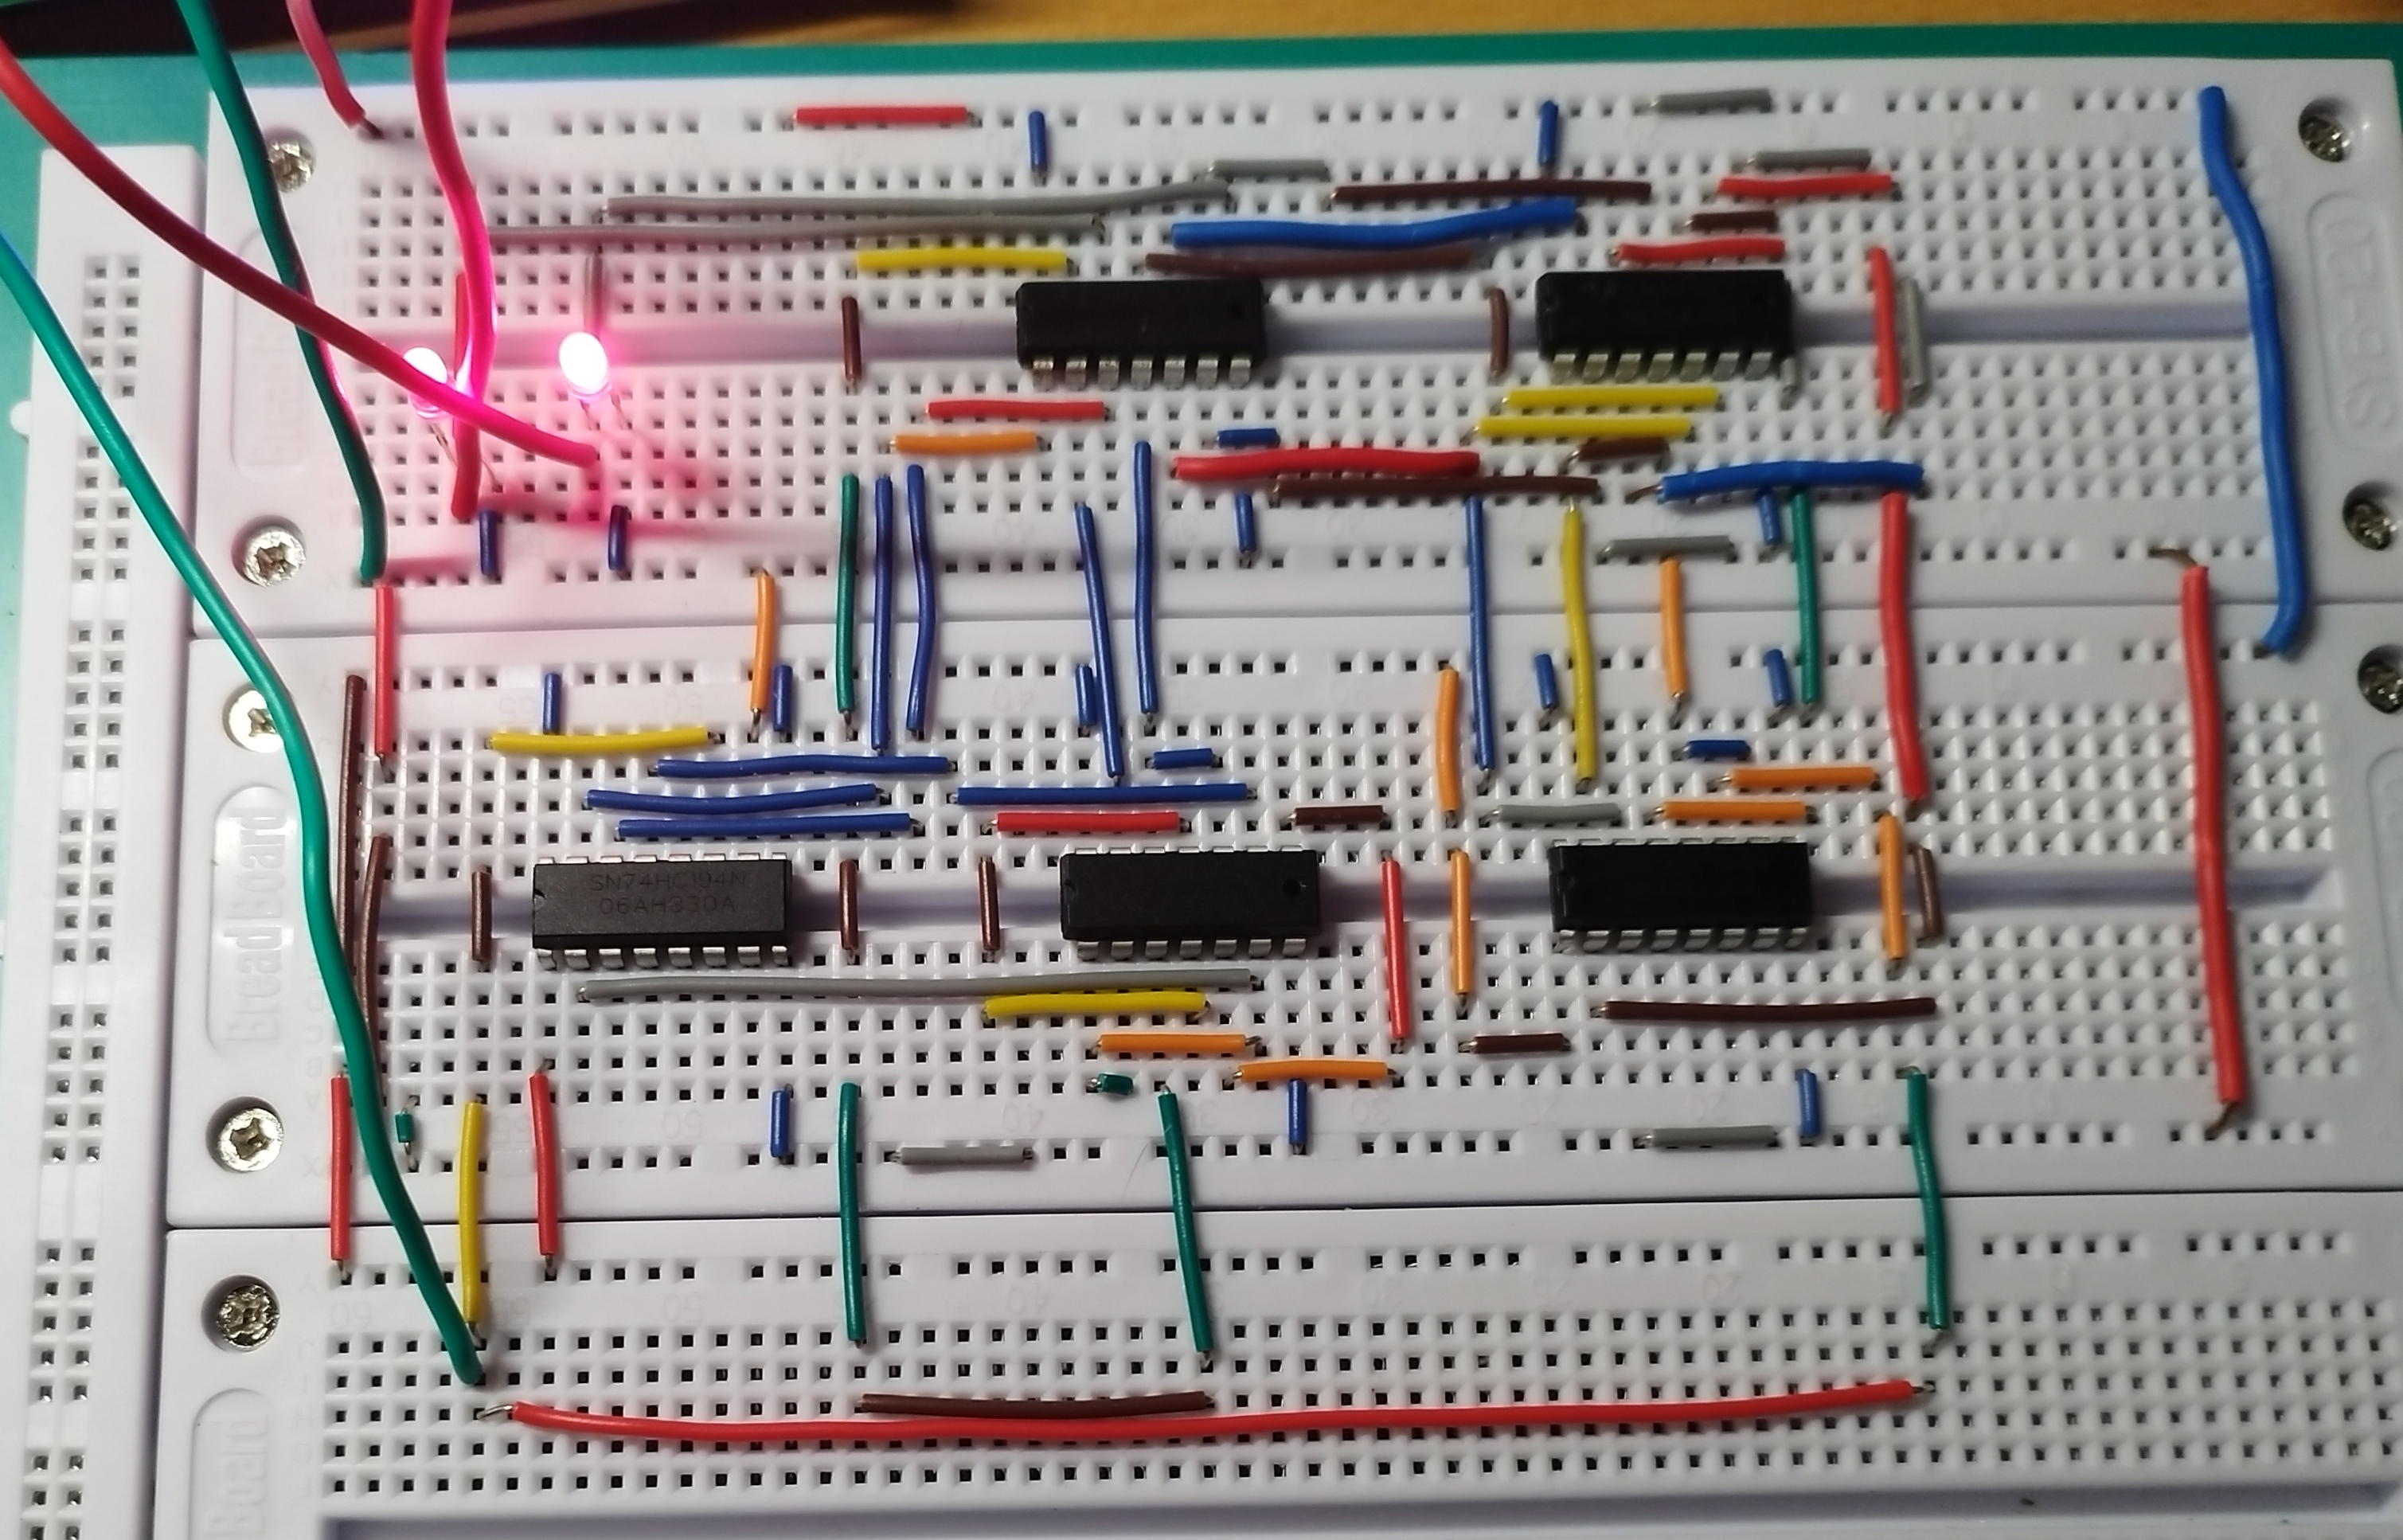
\includegraphics[width=0.5\textwidth]{点亮.jpg}
\end{figure}
\section{反思与总结}
本次实验总体来说较为顺利。但是在搭建实物电路时出现了以前出现过的低级错误:在利用环形计数器反馈函数输出高电平时直接接灯,这导致灯接通后直接到地,使得$D_{SR}$也接到地,反馈异常。本来想利用反馈函数作为输出减少接线,但为了避免上述情况,不得不接两个非,反而使接线变得更复杂。这样的问题在以后要避免。
\end{document}